\documentclass[12pt]{article}
\usepackage{adobeornaments}
\usepackage{textcsc}
\usepackage{xcolor}
\usepackage{fontspec}\definecolor{darkspringgreen}{rgb}{0.09, 0.45, 0.27}
\usepackage{titlesec}
\titleformat{\subsection}
  {\bfseries}{\thesection.\thesubsection}{1em}{\normalfont\bfseries}
\usepackage[hidelinks]{hyperref}
%\usepackage{fancyvrb}
\usepackage{hologo}
\usepackage{pdfpages}
\usepackage[british]{babel}
\usepackage[useregional]{datetime2}
\DTMlangsetup[en-GB]{ord=omit}
\definecolor{LightGray}{gray}{0.9}
%\usepackage{mathpazo}
\IfFontExistsTF{Palatine Parliamentary}{%
\setromanfont[SmallCapsFeatures={LetterSpace=10},
RawFeature={+calt,+hlig,+liga,+dlig,+onum,+pnum},
BoldFont={Palatine Parliamentary Bold},
ItalicFont={Palatine Parliamentary Italic}
]{Palatine Parliamentary Regular}
}{\setromanfont[RawFeature={+onum,+pnum}]{TeX Gyre PagellaX}}
\setmonofont[Scale=.9,BoldFont=Source Code Pro Bold]{Source Code Pro}

\usepackage{minted}
\date{\today\\\smallskip\ttfamily Version \adobeornamentsversionnumber}
\author{Elijah Z Granet\thanks{e-mail: \href{mailto:ezg21@cantab.ac.uk}{\ttfamily ezg21@cantab.ac.uk}}}

\title{\texttt{adobeornaments}:\\A package for typesetting ornaments in Adobe\textsuperscript{®️} Fonts}
\begin{document}
\maketitle
\tableofcontents
\clearpage
\section{Overview}
Several Adobe\textsuperscript{®️} fonts provide `hidden' ornaments, fleurons, and other typographic flourishes as additional features. These can be annoying to access in \LaTeX. This package provides any easy command to use the ornaments, and a guide to the individual ornaments to enable easy use (appended to this documentation and available separately in the package as \texttt{adobeornaments-list.pdf}).  \textcolor{red}{The fonts with these ornaments are sold by Adobe\textsuperscript{®️} and not provided with this package. You must purchase them separately for the package to work, or, in the case of Minion Pro only, obtain the free copy bundled with Adobe Reader.}
\section{Usage}
The package provides a single command 
{\color{darkspringgreen}\ttfamily\bfseries{%
\verb|\orn{$font}{$number}|%
}%
}%
.  The numbers of each ornament are provided in the aforementioned guide. The font options, as shown in the appendix, are:
\begin{center}
	\begin{tabular}{lr}
		\textbf{Font} & \textbf{Command}\\
Adobe Caslon Pro & \texttt{caslon}\\
Adobe Garamond Pro & \texttt{agp}\\
Adobe Jenson Pro & \texttt{jenson}\\
Arno Pro & \texttt{arno}	\\
Bickham Script Pro & \texttt{bickham}\\
Brioso Pro & \texttt{brioso}\\
Chaparral & \texttt{chaparral}\\
Cronos Pro & \texttt{cronos}\\
Garamond Premier Pro &  \texttt{gpp}\\\
Kepler Std & \texttt{kepler}\\
Minion Pro & \texttt{minion}\\
Warnock Pro & \texttt{warnock}\\
Silentium Pro & \texttt{silentium}\\
Voluta Script Pro & \texttt{voluta}\\
		
	\end{tabular}
	\end{center}
\clearpage
For example, the commands 
\begin{minted}[
framesep=2mm,
baselinestretch=1.2,
bgcolor=LightGray,
fontsize=\footnotesize,
breaklines,
firstnumber=last
]
{latex}
	\orn{minion}{1}\orn{caslon}{44}\orn{kepler}{31}
\end{minted}
Produce:
\begin{quote}
	\orn{minion}{1} \orn{caslon}{44}\orn{kepler}{31}\orn{bickham}{17}

\end{quote}


\normalfont
 

\section{Development}
Bugs, feature requests, \textit{etc}, should be submitted to the project's official Github page: (\url{github.com/ezgranet/adobeornaments}).
\section{Licence}
	This project is licensed under the \LaTeX\ Public Project Licence version 1.3\textit{c}. This documentation is copyright of the author but licensed under \textcsc{CC-BY-SA} 3.0.
	\clearpage 
\section{Implementation}
\begin{minted}[
frame=lines,
framesep=2mm,
baselinestretch=1.2,
bgcolor=LightGray,
fontsize=\footnotesize,
linenos,
breaklines,
firstnumber=last
]
{latex}
\def\adobeornamentsversionnumber{1.0.0}
\ProvidesPackage{adobeornaments}
[2023/05/13\adobeornamentsversionnumber\
 Command for ornaments in Adobe fonts]
% This work may be distributed and/or modified under the 
% conditions of the LaTeX Project Public License, either version 1.3c 
% of this license or (at your option) any later version.
% The latest version of this license is in
%   http://www.latex-project.org/lppl.txt
% and version 1.3c or later is part of all distributions of LaTeX 
% version 2005/12/01 or later.
%
% This work has the LPPL maintenance status `maintained'.
%
% The Current Maintainer of this work is Elijah Z Granet
%%%%%%%%%%%%%%%%%%%%%%%%%%%
% Warning that you need
% fontspec 
%%%%%%%%%%%%%%%%%%%%%%%%%%%
%%%%%%%%%%%%%%%%%%%%%%%%%%%
\RequirePackage{iftex}
\ifPDFTeX   {
    \PackageError{textcsc}
      {You are using pdfTeX but this package only works 
      \MessageBreak with XeTeX or LuaTeX}{}
    }
\fi
%obviously you need fontspec
\RequirePackage{fontspec}%
% if structure to stop error if someone only has *some* of the fonts
\IfFontExistsTF{Arno Pro}%
{%%%%%
\newfontfamily\arno[Scale=1.01]{Arno Pro}%%%%%
}{}%%%%%
\IfFontExistsTF{Minion Pro}{%%%%
\newfontfamily\minion[Scale=1.01]{Minion Pro}%%%%
}{}%%%
\IfFontExistsTF{Warnock Pro}%%%%%
{%%%%%
\newfontfamily\warnock[Scale=1.01]{Warnock Pro}
}%%%%%
{}
\IfFontExistsTF{Brioso Pro}{%
\newfontfamily\brioso[Scale=1.01]{Brioso Pro}%
}{}%
\IfFontExistsTF{Adobe Caslon Pro}{%
\newfontfamily\caslon[Scale=1.01]{Adobe Caslon Pro}%
}{}
\IfFontExistsTF{Adobe Jenson Pro}{%%%%
\newfontfamily\jenson[Scale=1.01]{Adobe Jenson Pro}%
}%
{}%%%%
\IfFontExistsTF{Adobe Garamond Pro}{%%%%%
\newfontfamily\agp[Scale=1.01]{Adobe Garamond Pro}%
}{}%%%%
\IfFontExistsTF{Kepler Std}{%%%%%
\newfontfamily\kepler[Scale=1.01]{Kepler Std}%%%%%
}%%%%
{}
\IfFontExistsTF{Voluta Script Pro}{%%%%%
\newfontfamily\voluta[Scale=1.01]{Voluta Script Pro}%%%%%
}%%%%
{}%
\IfFontExistsTF{Garamond Premier Pro}{%
\newfontfamily\gpp[Scale=1.01]{Garamond Premier Pro}%
}%
{}
\IfFontExistsTF{Cronos Pro}{%
\newfontfamily\cronos[Scale=1.01]{Cronos Pro}%
}{}
\IfFontExistsTF{Bickham Script Pro}{%
\newfontfamily\bickham[Scale=1.01]{Bickham Script Pro}%
}{}
\IfFontExistsTF{Chaparral Pro}{
\newfontfamily\chaparral%
[Scale=1.01]{Chaparral Pro}%
}{}
\IfFontExistsTF{Silentium Pro}{
\newfontfamily\silentium%
[Scale=1.01]{Silentium Pro}%
}{}
% xstring is required in order to apply if cases
\RequirePackage{xstring}
\newcommand{\orn}[2]{%
    \IfEqCase{#1}{%
{minion}%
{{\minion\addfontfeatures{Ornament=#2}•}}%
{arno}%
{{\arno\addfontfeatures{Ornament=#2}•}}%
{warnock}%
{{\warnock\addfontfeatures{Ornament=#2}•}}
{brioso}%
{{\brioso\addfontfeatures{Ornament=#2}•}}
{caslon}%
{{\caslon\addfontfeatures{Ornament=#2}•}}
{jenson}%
{{\jenson\addfontfeatures{Ornament=#2}•}}
{agp}%
{{\agp\addfontfeatures{Ornament=#2}•}}
{kepler}%
{{\kepler\addfontfeatures{Ornament=#2}•}}
{voluta}%
{{\voluta\addfontfeatures{Ornament=#2}•}}
{gpp}%
{{\gpp\addfontfeatures{Ornament=#2}•}}
{cronos}%
{{\cronos\addfontfeatures{Ornament=#2}•}}
{bickham}%
{{\bickham\addfontfeatures{Ornament=#2}•}}
{chaparral}%
{{\chaparral\addfontfeatures{Ornament=#2}•}}
{silentium}%
{{\silentium\addfontfeatures{Ornament=#2}•}}
        % you can add more cases here as desired
    }[\PackageError{orn}{Undefined font: #1}{}]%
}%

\end{minted}


\section{Version History}
\subsection{\texttt{1.0.1}}

\ttfamily 15 May 2023: Fix typo in readme

\subsection{\texttt{1.0.0}}

\ttfamily 14 May 2023: Package creation
\clearpage
\pagestyle{empty}\addcontentsline{toc}{section}{Appendix: Ornaments List}

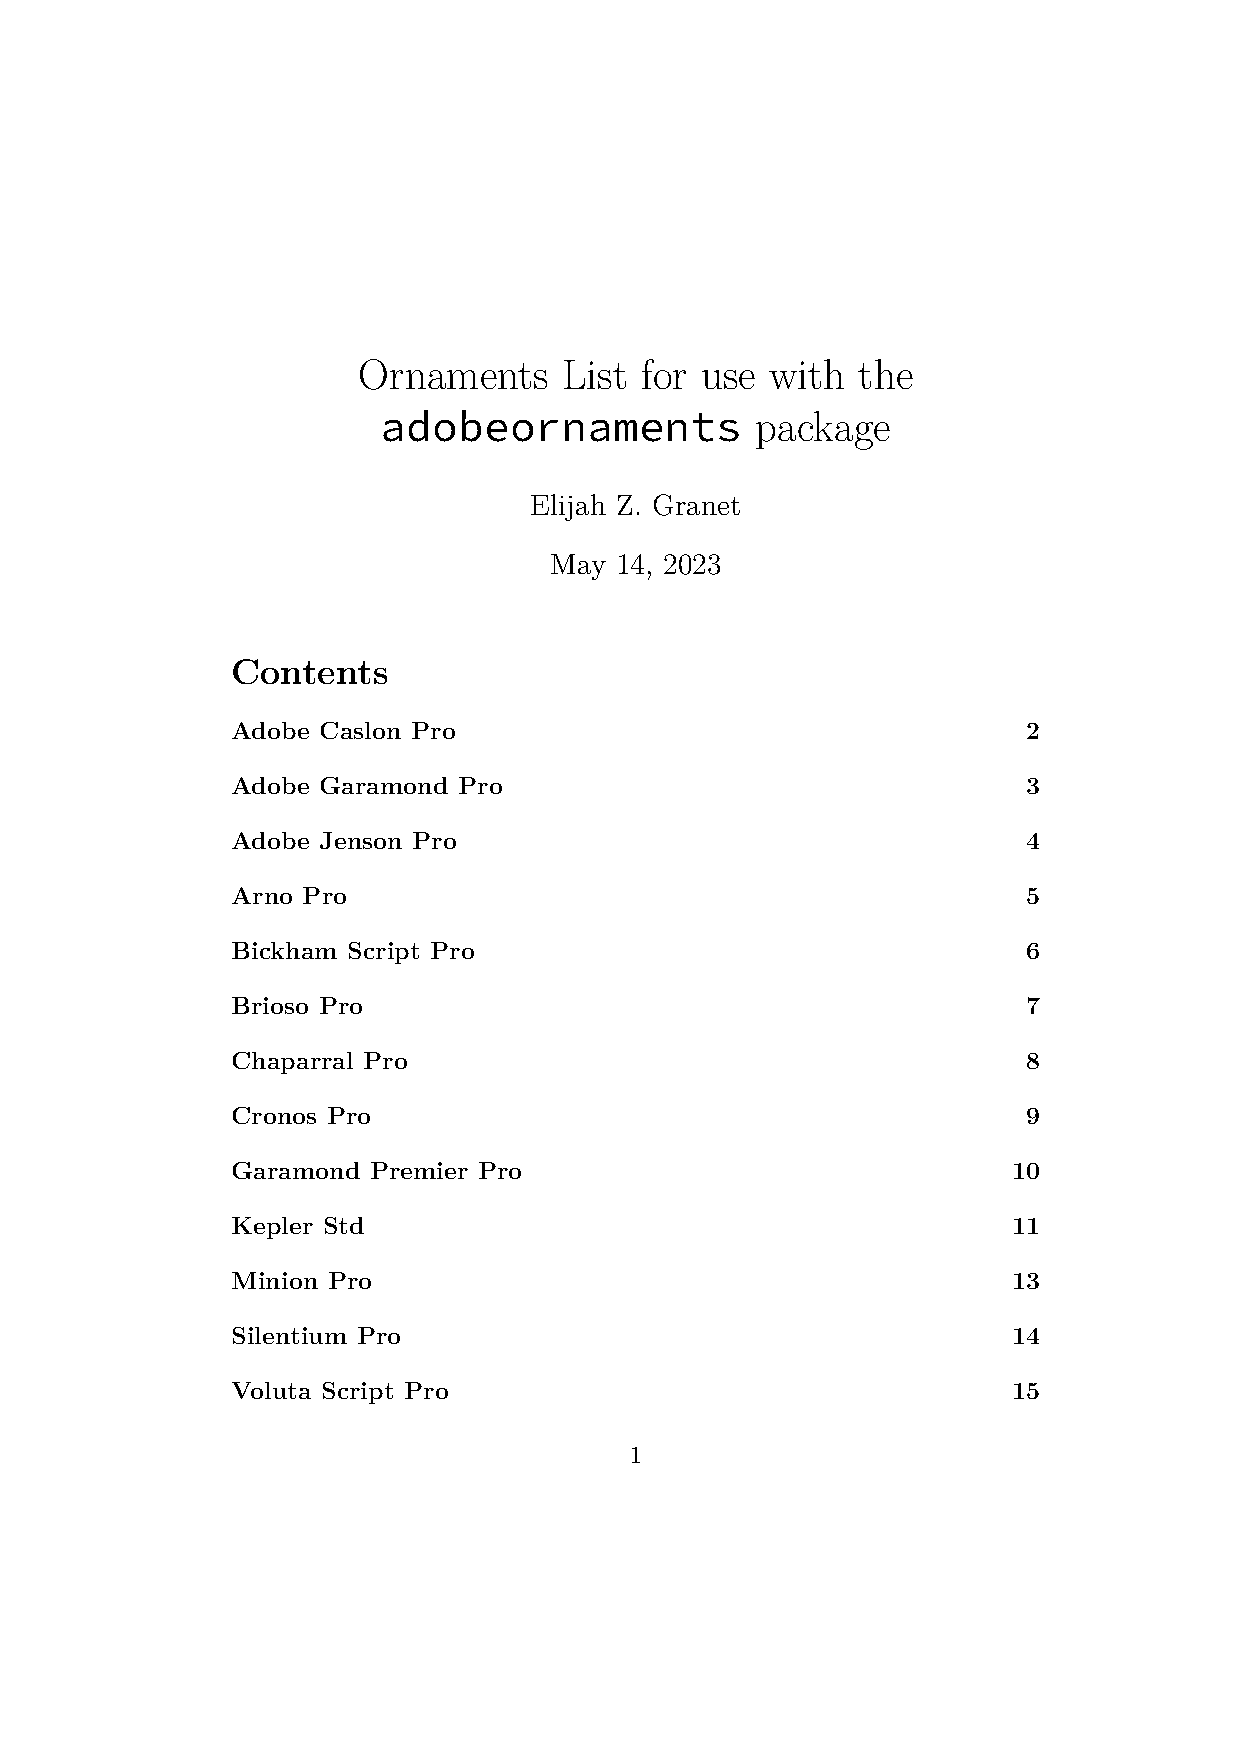
\includepdf[pages=-]{adobeornaments-list.pdf}

	
\end{document}